\documentclass{article}

\usepackage{packages}
\usepackage{environments}
\usepackage{commands}

\begin{document}

\title{Typing Analysis}
\author{Dima Trushin}
\date{}
	
\maketitle
\tableofcontents

\section{General information}

The application uses Qt environment as an ecosystem. It does not use RTTI but uses exceptions. All components of the program must be inside NSApplication namespace. Nested namespaces should be placed in a subfolder of the project.

\section{Addressable objects}

I use term addressable object. It means an object that can be referenced by other objects. There are several types of addressable objects:
\begin{enumerate}
\item QObject
\item CApplicationImpl
\item Observer/Observable (TO DO)
\end{enumerate}
Addressable objects must be created on heap via \verb"std::make_unique" or similar mechanism. An exception to this rule: you may create an addressable object inside another addressable object.

\section{Exceptions}

The strategy is to catch exception, show a message, and die. Since Qt environment is not totally exception safe, it is not allowed to throw exceptions in an event loop. If a QObject requires to throw an exception and terminate the program it sends a signal to QApp, QApp shows a message, and terminates execution (TO DO).

\section{Application Structure}

CApplication object initialize all required resources for the application including the ones to interact with Qt ecosystem. It may throw an exception while constructing. In order to minimize stack usage CApplication contains \verb"std::unique_ptr" to CApplicationImpl (it is addressable object). CApplicationImpl consists of four parts:
\begin{enumerate}
\item \textbf{CApplicationGlobals}. Its purpose is to initialize global resources, e.g., timers, loggers, thread pools, etc. Application initializes all global resources (basically singletons) at the start. This allows not to wast time on the first call. Also, it is inconvenient to initialize timers via the first call.
\item \textbf{CApplicationKernel}. Its purpose is to initialize the kernel of the application. The kernel does not depend on the GUI and uses MVC via observer pattern to interact with GUI.
\item \textbf{CApplicationGUI}. Its purpose is to provide View wrappers over Qt resources compatible with MVC pattern.
\item \textbf{CApplicationImpl}. Its purpose is to connect the kernel and the GUI via MVC.
\end{enumerate}
The order of construction is ensured by the inheritance mechanism.
\begin{center}
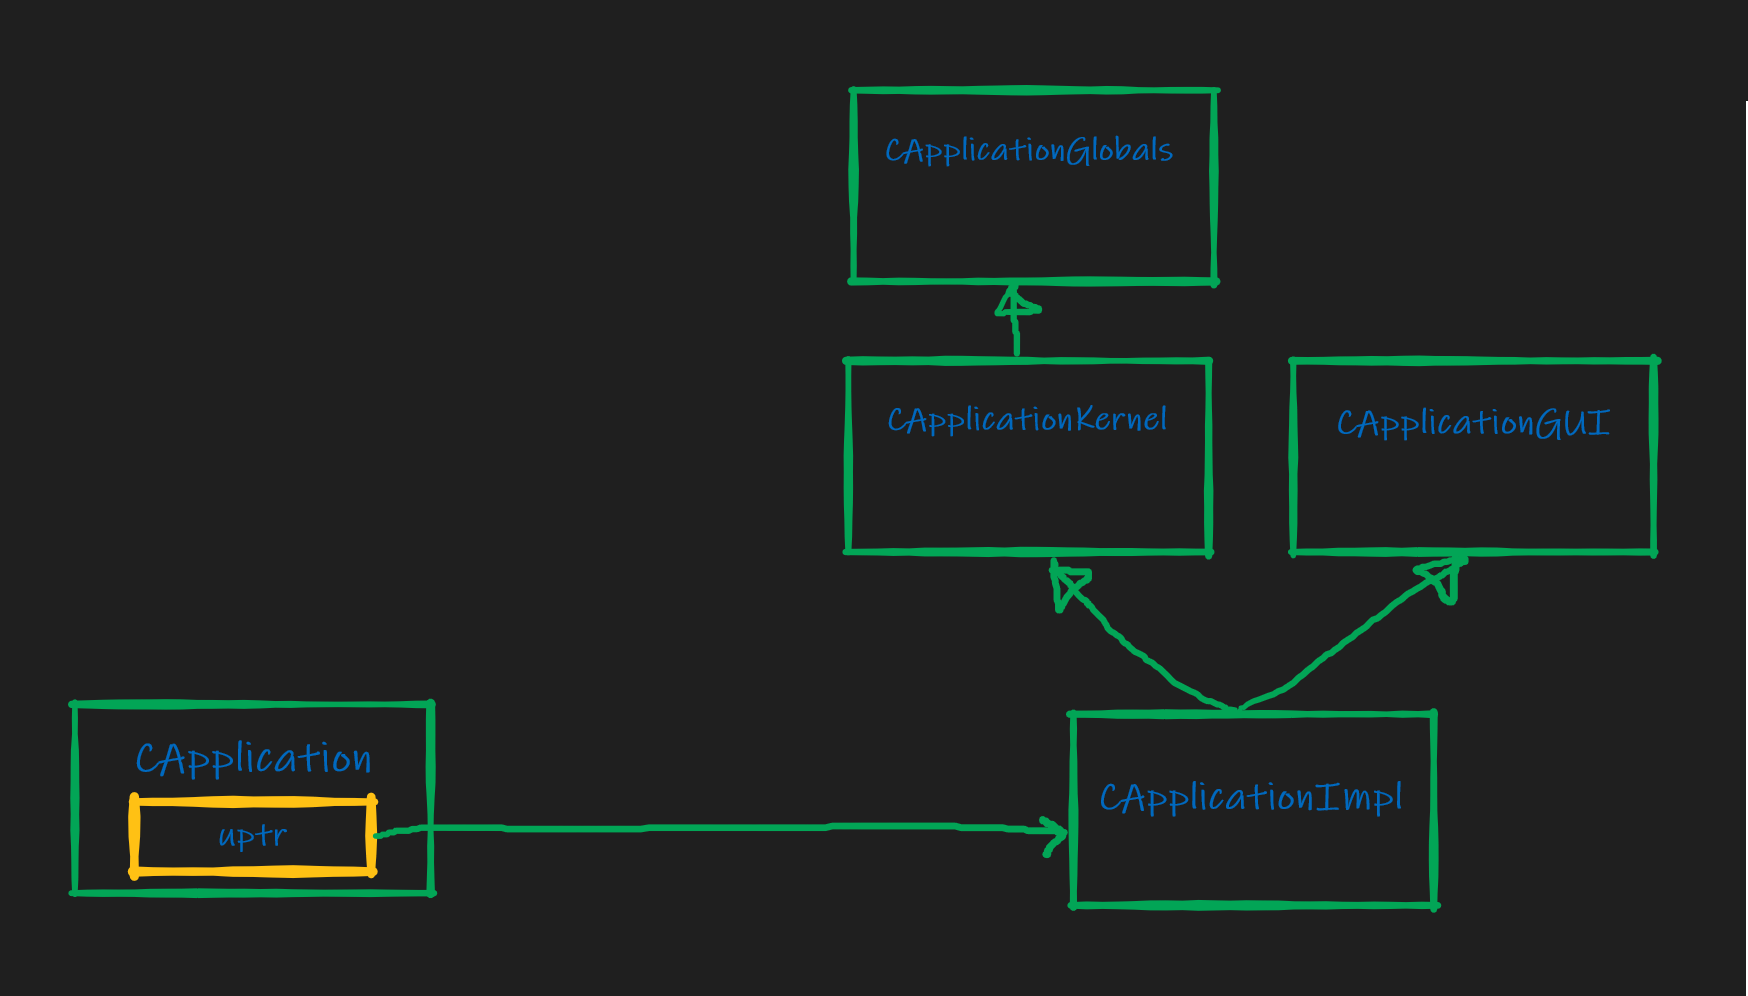
\includegraphics[scale = 0.3]{Figures/CApplicationStructure.png}
\end{center}
	
\end{document}
